\section{Machine Learning Techniques}
\label{sec:ml-techniques}
\subsection{Traditional Machine Learning Techniques}
\label{subsec:concepts-traditional-techniques}
\begin{frame}{\insertsubsection}
    \begin{figure}
        \centering
        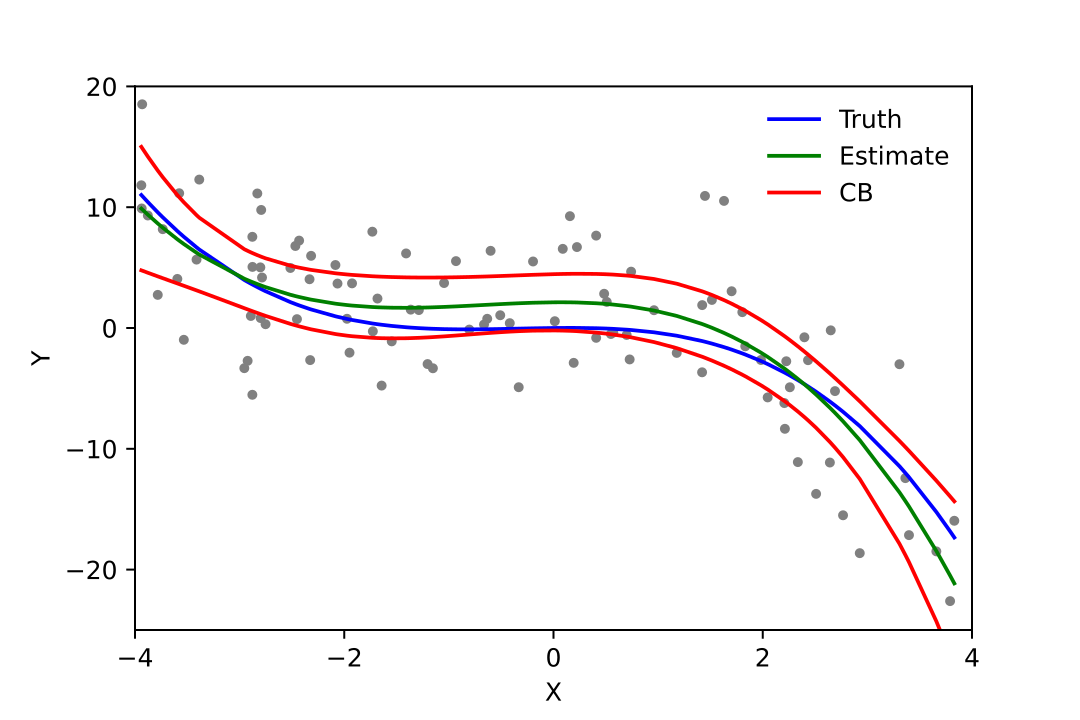
\includegraphics[width=0.8\textwidth]{media/Polyreg_scheffe.png}
        \caption{Polynomial Regression~\cite{Skbkekas2009}}
    \end{figure}
\end{frame}
%
%
\begin{frame}{\insertsubsection}
    \begin{figure}
        \centering
        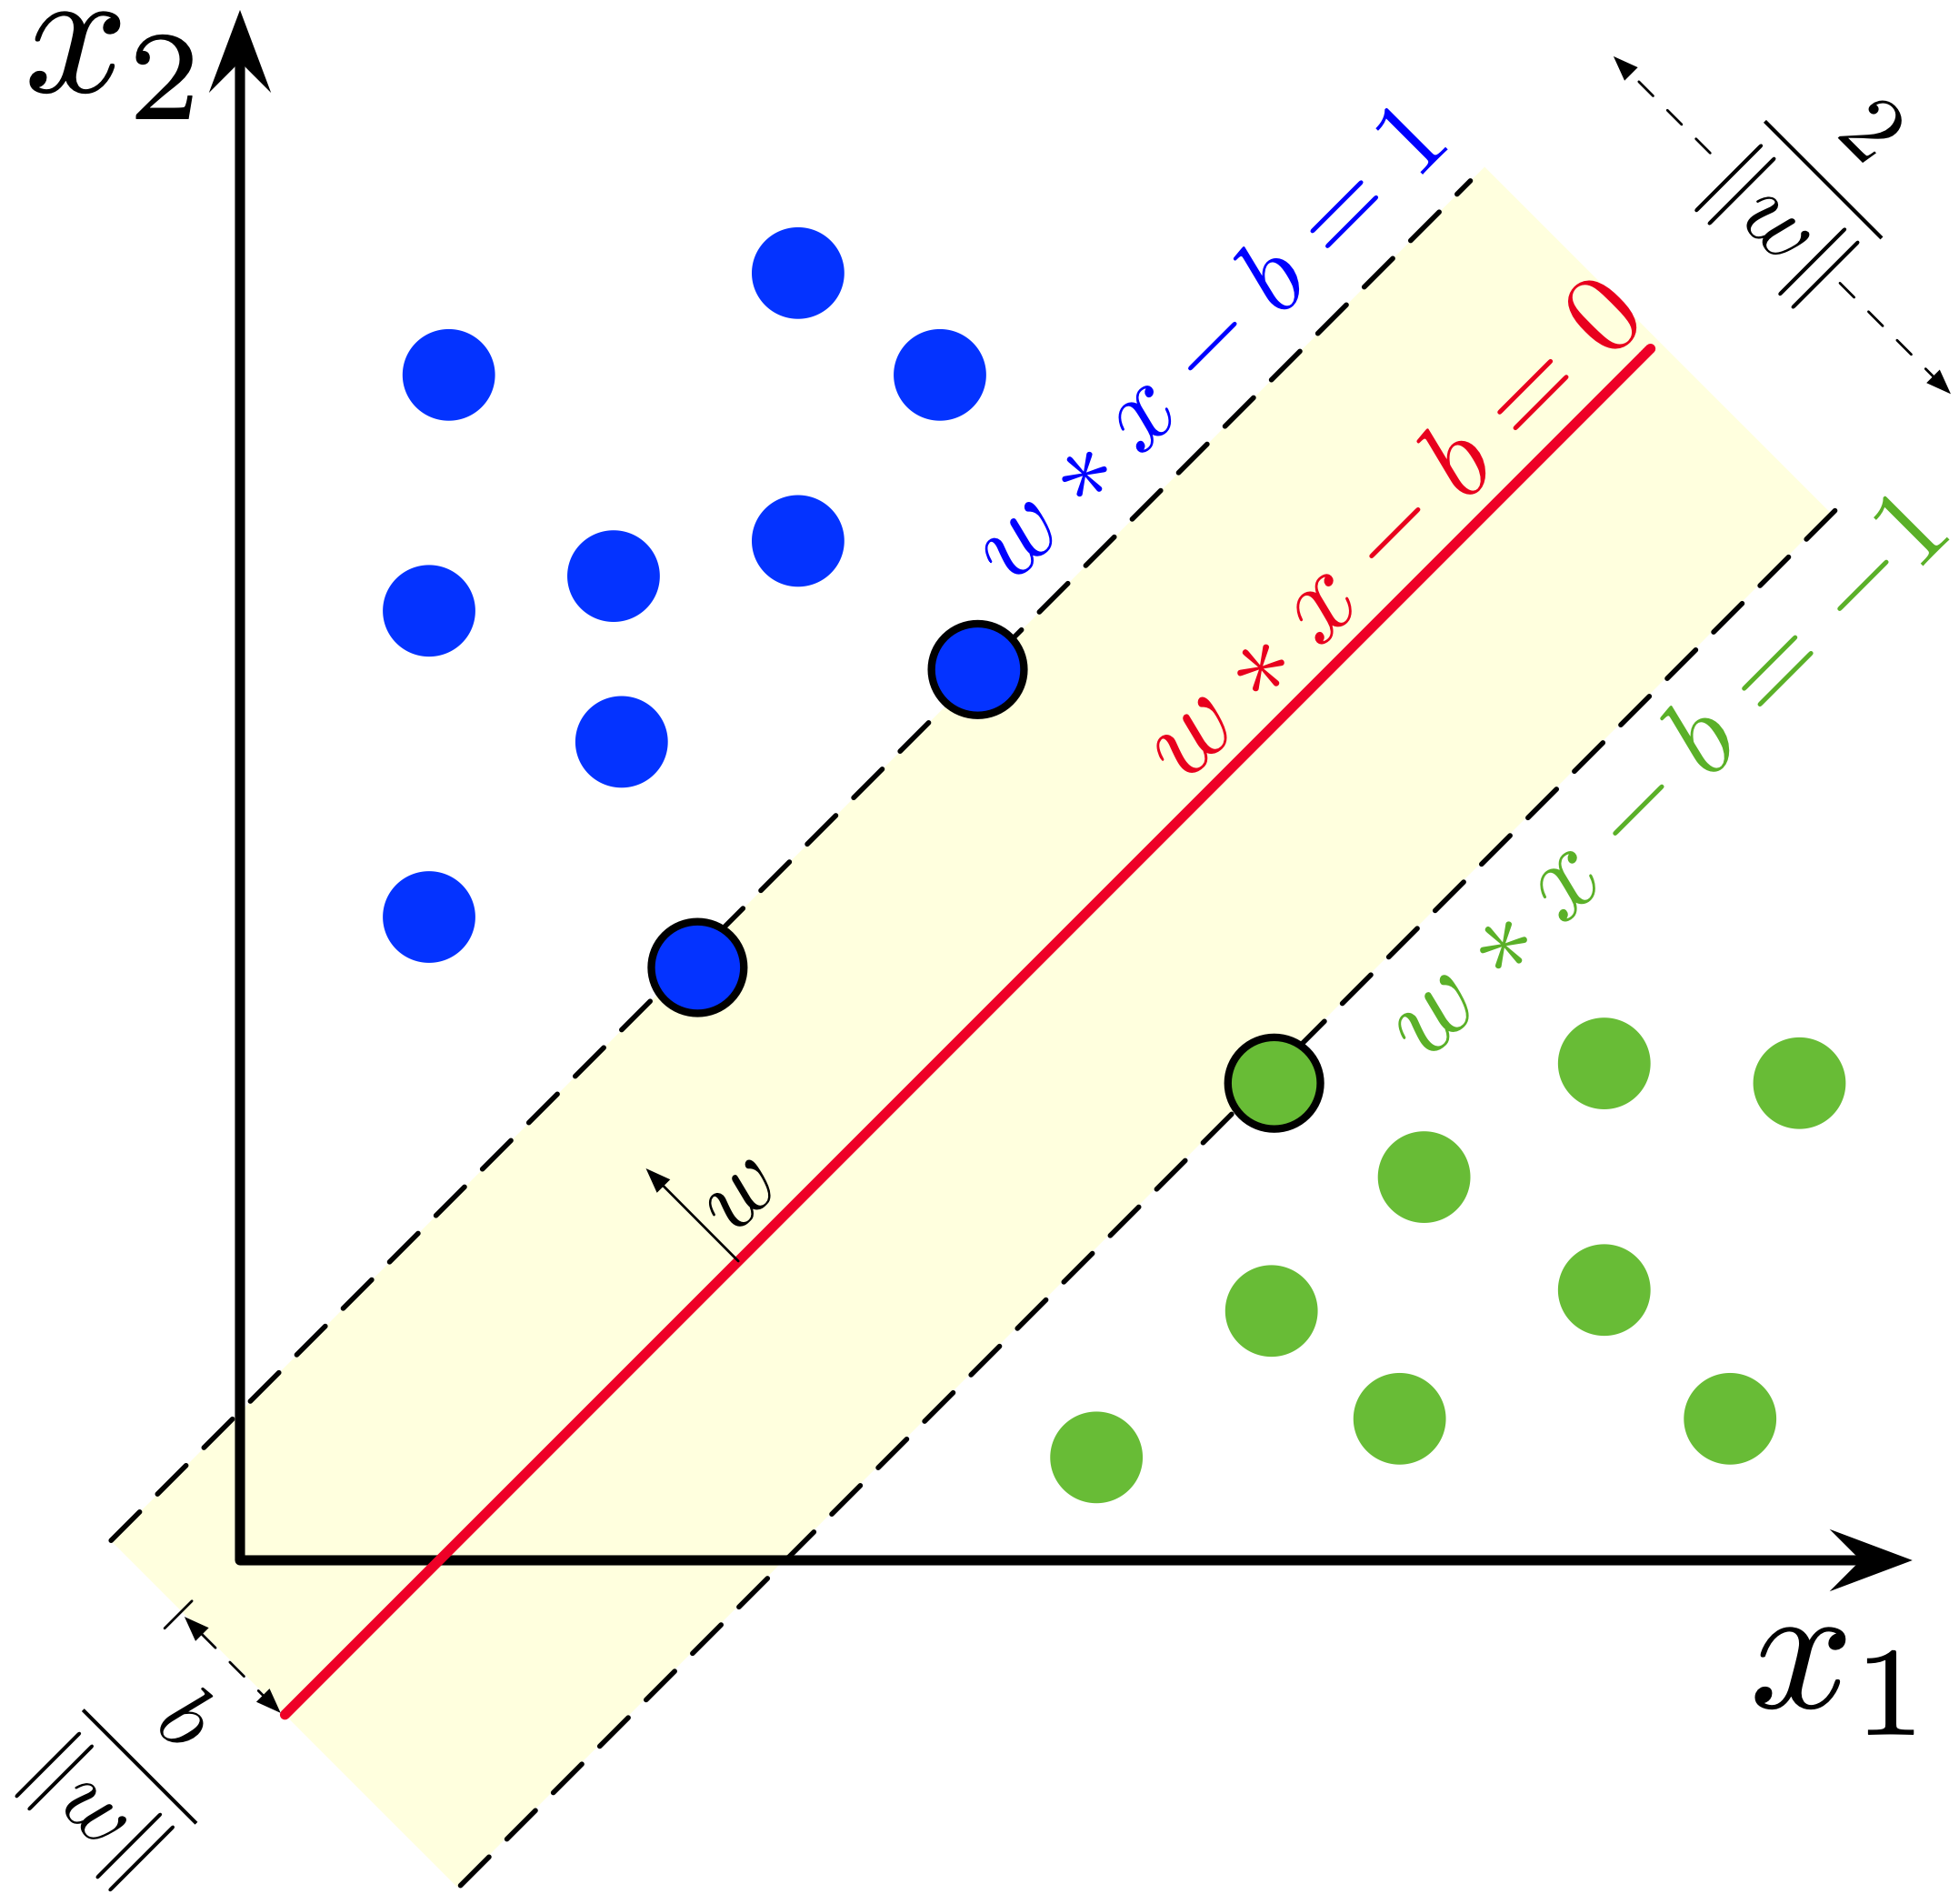
\includegraphics[width=0.6\textwidth]{media/SVM_margin.png}
        \caption{Support Vector Machine~\cite{Larhmam2018}}
    \end{figure}
\end{frame}
%
%
\begin{frame}{\insertsubsection}
    \begin{itemize}
        \item Traditional machine learning routines should be preferred over neural networks
        \item Deep learning can be powerful (and trendy)
        \item[] However, currently still limited in applicability
        \item[] Requires lots of data $\Rightarrow$ often not present
        \item Traditional Methods are faster to develop and test
        \item[] They typically expect same number of features with each datapoint
        \item[] $\Rightarrow$ Padding and Windowing are methods to circumvent this
    \end{itemize}
\end{frame}
%
%
